\documentclass[../main.tex]{subfiles}
\begin{document}
Poisson's equation is
\begin{equation}\label{eq:Poisson}
\Delta\upvarphi=f
\end{equation}
where $\Delta$ is the Laplace operator, and $f$ and $\upvarphi$ are real or complex-valued functions. In Euclidean space, the Laplace operator is often denoted as $\nabla^2$ and so Poisson's equation is frequently written as
\begin{equation}\label{eq:Poisson2}
\nabla^2\upvarphi=f
\end{equation}
In three-dimensional Cartesian coordinates, it takes the form
\begin{equation}\label{eq:Poisson3}
\Big(\frac{\partial^2}{\partial x^2} + \frac{\partial^2}{\partial y^2}+\frac{\partial^2}{\partial z^2}\Big)\upvarphi(x,y,z) = f(x,y,z)
\end{equation}
When $f=0$ we have Laplace's Equation.

%%%%%%%%%%%%%%%%%%%%%%%%%%%%%%%%%%%
\subsection{Problem Statement}
Consider the second-order differential equation
\begin{equation}\label{eq:ProblemStatement}
\frac{\partial^2}{\partial x^2}\upvarphi(x) = f(x)
\end{equation}
Use the finite difference method to approximate the partial differential equation over the interval $x\in(a,b)$ assuming a uniform spatial discretization $\Delta x$. $\upvarphi$ need not be twice-differentiable over $\mathbb{R}$ but only over the interval $x\in(a,b)$. \color{red}Although conceptually easy, finite differences are difficult to apply over domains with heterogenous composition?
\color{black}

%%%%%%%%%%%%%%%%%%%%%%%%%%%%%%%%%%%
\subsection{Finite-Difference Method}
The Finite-Difference Method (FDM) is a numerical procedure which solves a PDE by:
\begin{itemize}
	\item Discretizing the continuous physical domain into a discrete \textbf{finite difference grid}
    \item Approximating the individual exact partial derivatives in the PDE by algebraic \textbf{finite difference approximations (FDAs)}
    \item Substituting the FDAs into the PDE to obtain an algebraic \textbf{finite difference equation (FDE)}
    \item Solving the resulting algebraic FDEs for the dependent variable.
\end{itemize}

\subsubsection{Finite Difference Grid}
Consider the following one-dimensional domain D(x),
\begin{figure}[H]\label{fig:Domain}
\center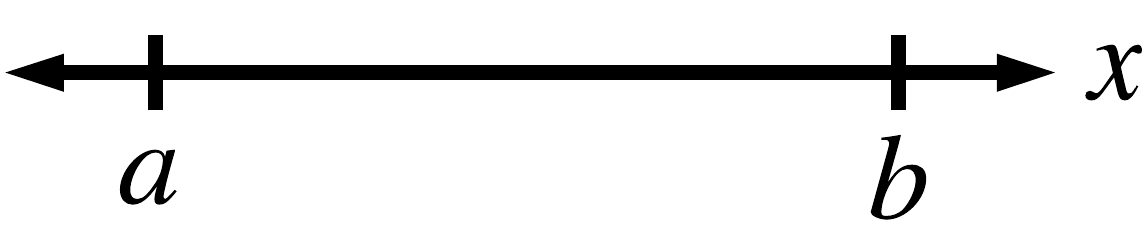
\includegraphics[scale = 0.5]{../image.png}
\end{figure}
\noindent which must be covered by a one-dimensional grid of lines (figure \ref{fig:Domain}). Let $x_i = a + (i-1)\Delta x$, $f(x_i) = f_i$, $f_x(x_i) = f_x|_i$ and $f_{xx}(x_i) = f_{xx}|_i$.

\begin{figure}[H]
	\center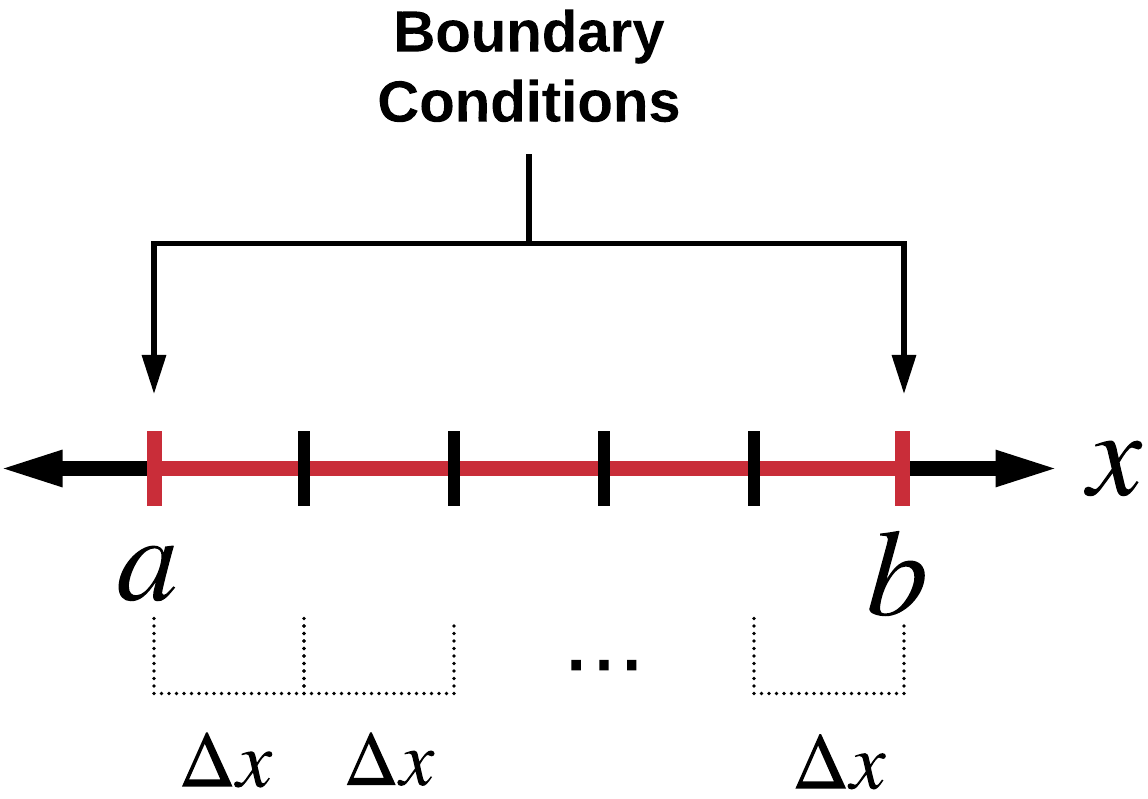
\includegraphics[scale=0.5]{../image1.png}
    \caption{Discrete difference grid with a uniform spatial discretization of $\Delta x$}
    \label{fig:SolutionDomain}
\end{figure}

\subsubsection{Finite Difference Approximations}
\color{red}\textbf{Note:} For elliptic PDEs containing only second derivatives, there are no preferred physical informative propagation paths. Thus, centered-space finite difference approximations should be used for the second-order spatial derivatives in the Laplace equation and the Poisson equation.\color{black}

\vspace{1em}
\noindent\textbf{Exact Solution:} $\bar{f}(x)$

\noindent\textbf{Approximate Solution:} $f(x)$

\vspace{1em}
\noindent Consider the Taylor Series expansion of $\bar{f}_{i-1}$ and $\bar{f}_{i-1}$ using $i$ as the base point gives
\begin{equation}\label{eq:taylor1}
\bar{f}_{i+1} = \bar{f}_i+\bar{f}_x|_i\Delta x + \frac{1}{2}\bar{f}_{xx}|_i(\Delta x)^2 +\cdots
\end{equation}
\begin{equation}\label{eq:taylor2}
\bar{f}_{i-1} = \bar{f}_i-\bar{f}_x|_i\Delta x + \frac{1}{2}\bar{f}_{xx}|_i(\Delta x)^2 -\cdots
\end{equation}
Adding the first three terms of equations (\ref{eq:taylor1}) and (\ref{eq:taylor2}) (up to the second partial) we can approximate $\bar{f}_{xx}|_i$,
\begin{equation}\label{eq:SecondOrderApprox}
f_{xx}|_i= \frac{f_{i+1} - 2f_i + f_{i-1}}{(\Delta x)^2}
\end{equation}
which serves as our second-order centered-difference approximation at $i$.

%%%%%%%%%%%%%%%%%%%%%%%%%%%%%%%%%%%%%%%%%%%%%%%%%%%%%%%%%%%%%%%%%%%%%%%%%%%%%%%%%%%%%%%%%%
\subsection{Finite Difference Solution of the Laplace Equation}
If $f(x) = 0$ in equation (\ref{eq:ProblemStatement}) of our problem statement, we have the Laplace Equation
\begin{equation}\label{eq:Laplace}
\frac{\partial^2}{\partial x^2}\upvarphi(x) = \bar{f}_{xx} = 0
\end{equation}
Substituting equation (\ref{eq:SecondOrderApprox}) yields
\begin{equation}\label{eq:Laplace2}
\frac{f_{i+1} - 2f_i + f_{i-1}}{(\Delta x)^2} = 0
\end{equation}
while solving for $f_i$ gives
\begin{equation}\label{eq:Laplace3}
f_i = \frac{f_{i-1}+f_{i+1}}{2}
\end{equation}
Simply stated, the solution at every point is the arithmetic average of the solutions of the neighboring points. \textbf{Note:} This result applies only to the Laplace equation (i.e. no nonhomogeneous term). 

Let $u_i$ represent the approximation of $\upvarphi (x_i)$ in (\ref{eq:Laplace}). Assuming the uniform spatial discretization yields $n$ partitions, we have the following system of equations,
\begin{align}
u_2 &= \frac{a + u_3}{2}\nonumber\\
u_3 &= \frac{u_2 + u_4}{2}\nonumber\\
&\vdots\\
u_{n-2} &= \frac{u_{n-3} + u_{n-1}}{2}\nonumber\\
u_{n-1} &= \frac{u_{n-2} + b}{2}\nonumber
\end{align}
or
\begin{align*}
 (2)u_2 - (1)u_3 + (0)u_4 + & \cdots + (0)u_{n-3} + (0)u_{n-2} + (0)u_{n-1} = a\\
-(1)u_2 + (2)u_3 - (1)u_4 + & \cdots + (0)u_{n-3} + (0)u_{n-2} + (0)u_{n-1} = 0\\
& \vdots\\ 
 (0)u_2 + (0)u_3 + (0)u_4 + & \cdots - (1)u_{n-3} + (2)u_{n-2} - (1)u_{n-1} = 0\\
 (0)u_2 + (0)u_3 + (0)u_4 + & \cdots + (0)u_{n-3} + (1)u_{n-2} + (2)u_{n-1} = b
\end{align*}
which when expressed in matrix form 
\[
\begin{bmatrix}
    2		&	-1		&	0		&	\cdots	&0&	0		&	0\\
    -1		&	2		&	-1		&	\cdots	&0&	0		&	0\\
    \ddots	&	\ddots	&	\ddots	&	\ddots	&\ddots&	\ddots	&	\ddots\\
    0		&	0		&	0		&	\hdots	&-1&	2		&	-1\\
    0		&	0		&	0		&	\hdots	&0&	-1		&	2
\end{bmatrix}
\cdot
\begin{bmatrix}
    u_2\\u_3\\\vdots\\u_{n-2}\\u_{n-1}
\end{bmatrix}
=
\begin{bmatrix}
a\\0\\\vdots\\0\\b
\end{bmatrix}
\]

%%%%%%%%%%%%%%%%%%%%%%%%%%%%%%%%%%%%%%%%%%%%%%%%%%%%%%%%%%%%%%%%%%%%%%%%%%%%%%%%%%%%%%%%%%
\subsection{Finite Difference Solution of the Poisson Equation}
Similar to equation (\ref{eq:Laplace}) except that $f(x) \ne 0$. Let $f(x) = g(x)$, then we have
\begin{equation}
\frac{\partial^2}{\partial x^2}\upvarphi(x) = \bar{f}_{xx} = g(x)
\end{equation}
For $g(x) \ne 0$, equations (\ref{eq:Laplace2}) and (\ref{eq:Laplace3}) become
\begin{equation}
\frac{f_{i+1} - 2f_i + f_{i-1}}{(\Delta x)^2} = g(x)
\end{equation}
\begin{equation}
f_i = \frac{f_{i-1}+f_{i+1}-g_i(\Delta x)^2}{2}
\end{equation}
which yields a similar system of equations when represented in matrix form gives
\[
\begin{bmatrix}
    2		&	-1		&	0		&	\cdots	&0&	0		&	0\\
    -1		&	2		&	-1		&	\cdots	&0&	0		&	0\\
    \ddots	&	\ddots	&	\ddots	&	\ddots	&\ddots&	\ddots	&	\ddots\\
    0		&	0		&	0		&	\hdots	&-1&	2		&	-1\\
    0		&	0		&	0		&	\hdots	&0&	-1		&	2
\end{bmatrix}
\cdot
\begin{bmatrix}
    u_2\\u_3\\\vdots\\u_{n-2}\\u_{n-1}
\end{bmatrix}
=
\begin{bmatrix}
a-g_2(\Delta x)^2\\-g_3(\Delta x)^2\\\vdots\\-g_{n-2}(\Delta x)^2\\b-g_{n-1} (\Delta x)^2
\end{bmatrix}
\]

%%%%%%%%%%%%%%%%%%%%%%%%%%%%%%%%%%%%%%%%%%%%%%%%%%%%%%%%%%%%%%%%%%%%%%%%%%%%%%%%%%%%%%%%%%
\subsection{Derivative Boundary Conditions}
Consider equation (\ref{eq:ProblemStatement}) in our problem statement with unknown boundary point conditions but known derivatives. We approximate these unknown boundary points using their derivatives and adjacent interior point. Recall the approximation for $f_I$,
\begin{equation}
f_{I+1} +f_{I-1}-2f_I = g_I (\Delta x)^2
\end{equation}
for either $f_{I-1}$ or $f_{I+1}$ unknown (depending on which boundary point we are considering). Using the difference formula
\begin{equation}\label{eq:approximation2}
f_x|_I = \frac{\bar{f}_{I+1}-\bar{f}_{I-1}}{2\Delta x}
\end{equation}
and solving for either $f_{I-1}$ or $f_{I+1}$ (again depending on which boundary point we are considering) we arrive at
\begin{align}
2f_{I-1}-2f_I=-2\bar{f}_x|_I \Delta x + g_I (\Delta x)^2\\
2f_{I+1}-2f_I=-2\bar{f}_x|_I \Delta x + g_I (\Delta x)^2
\end{align}
which can be explicitly solved for $f_{I-1}$ or $f_{I+1}$. \textbf{Note:} $\bar{f}_x|_I$ and $g_I$ in these equations are not necessarily the same.
\color{red}The original form of equation (\ref{eq:approximation2}) is
\begin{equation}\label{eq:MysteryApproximation}
f_x|_i = \frac{f_{i+1} - f_{i-1}}{2\Delta x} - \frac{1}{6}f_{xxx}(\zeta)(\Delta x)^2
\end{equation}
I easily see how equation (\ref{eq:approximation2}) was derived but not equation (\ref{eq:MysteryApproximation}). Is this derived from the Taylor Series?
\color{black}

\subsection{Iterative Methods of Solution}
\subsubsection{Jacobi Iteration}
\subsubsection{Gauss-Seidel Iteration}
\subsubsection{Successive-over-relaxation (SOR) }

\end{document}
